\documentclass[10pt]{beamer}
\usetheme{jambro}

\title[]{Consumo, investimento e curva IS}
\author[]{Paulo Victor da Fonseca}
\date{02 de maio de 2023}

\hypersetup{
    colorlinks = true,
    urlcolor = teal,
    linkcolor = teal    
}
\usepackage[portuguese]{babel}
\usepackage{subfig}
\usepackage{emoji}
\usepackage{hyperref}

\begin{document}

\begin{frame}[plain]
    \titlepage{
        \begin{center}
            \begin{minipage}{0.8\textwidth}
                \centering
            \end{minipage}
        \end{center}}
\end{frame}

\begin{frame}{Sumário}
    \tableofcontents
\end{frame}

\section{Introdução}
\begin{frame}
    {Introdução}
    \NB{Aulas passadas: introduzimos modelos de consumo e investimento que levam em consideração comportamento \emph{forward-looking} dos agentes\bigskip
    
    Expectativas a respeito da renda e lucros futuros possuem papel importante nas decisões de gastos de firmas e famílias\bigskip

    Também vimos evidências empíricas de consumo agregado e investimento que mostram a importância de restrições de créditos para famílias e firmas}\bigskip

    \emoji{warning}\textcolor{purple}{Quais são as implicações destes fatores para a curva IS?}
\end{frame}

\begin{frame}
    {Introdução}
    \begin{itemize}
        \item Curva IS simples derivada anteriormente:
        \begin{eqnarray}
            y &=& \kappa(c_0 + a_0 + G) - \kappa a_1 r, \nonumber \\
            &=& A - ar, \label{aula9_eq1}
        \end{eqnarray}
        onde $A \equiv \kappa(c_0 + a_0 + G)$, $a \equiv \kappa a_1$ e $\kappa$ é o multiplicador\bigskip
        \item Quando o multiplicador é elevado, a IS é mais plana, o que aumenta o impacto sobre o produto de uma variação na taxa real de juros\bigskip
        \item Além disso, também aumenta o impacto sobre o produto agregado de um deslocamento em $c_0, a_0$ ou $G$ para uma dada taxa de juros\bigskip
        \item O que deixa claro que o tamanho do multiplicador é importante para a compreensão tanto da política fiscal quanto monetária
    \end{itemize}
\end{frame}

\begin{frame}
    {Introdução}
    \begin{itemize}
        \item Desde CFG2008, tem havido muito debate acerca do tamanho empírico dos multiplicadores no contexto da utilização de estímulos fiscais como resposta a períodos de recessão\bigskip
        
        \emoji{warning} Cabe ressaltar que não existe uma resposta simples à questão: qual o tamanho do multiplicador?\bigskip
        
        \item A resposta depende das características da economia considerada e do contexto no qual, e.g., o estímulo fiscal é aplicado
    \end{itemize}
\end{frame}

\begin{frame}
    {Introdução}
    \begin{figure}
        \centering
        \href{https://www.aeaweb.org/articles?id=10.1257/aer.100.2.30}{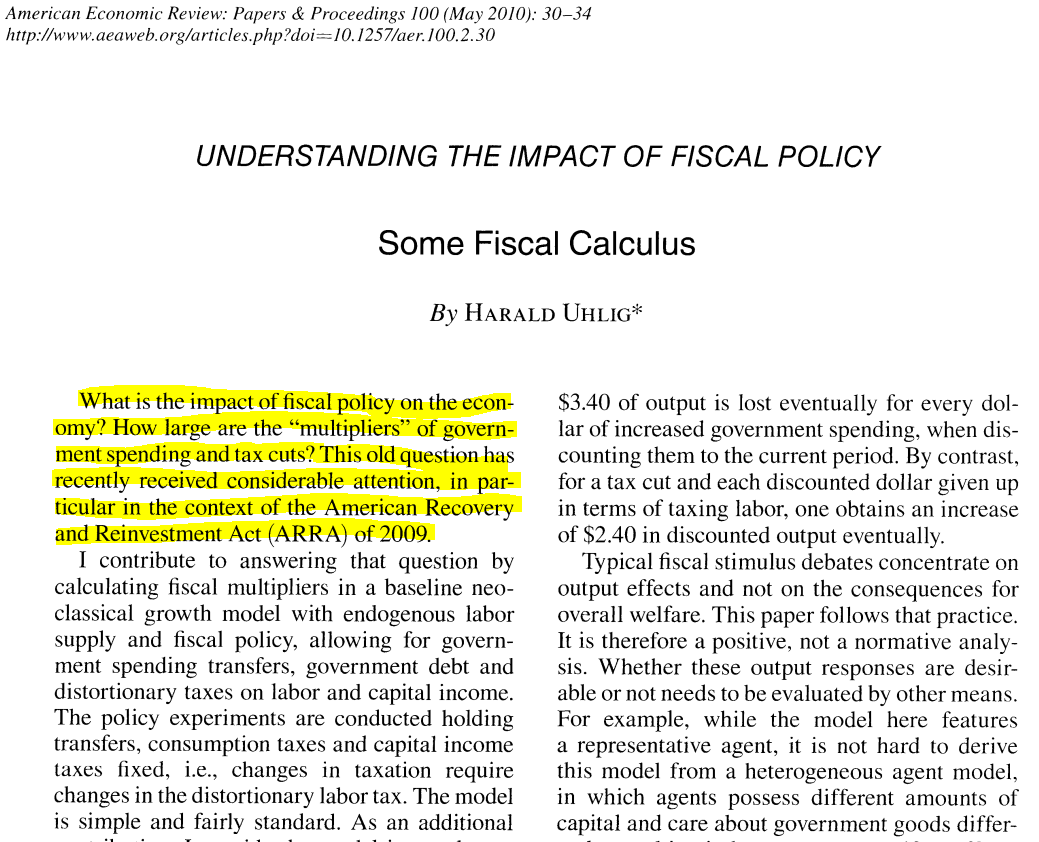
\includegraphics[width=0.6\textwidth]{./figures/aula9_fig4.PNG}}
    \end{figure}
\end{frame}

\begin{frame}{Introdução}
    \begin{tabular}{cc}        
        \begin{tabular}{c}
            \parbox{0.5\linewidth}{
            \href{https://www.aeaweb.org/articles?id=10.1257/jep.33.2.89}{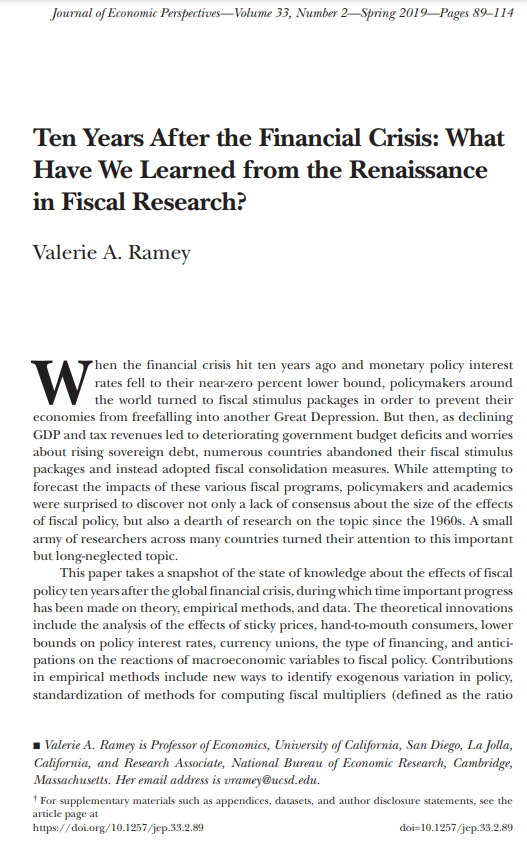
\includegraphics[width=5cm]{./figures/aula9_fig2.PNG}}            
            }
        \end{tabular}
         & \begin{tabular}{c}
            \parbox{0.5\linewidth}{
            \href{https://www.aeaweb.org/articles?id=10.1257/jep.33.2.89}{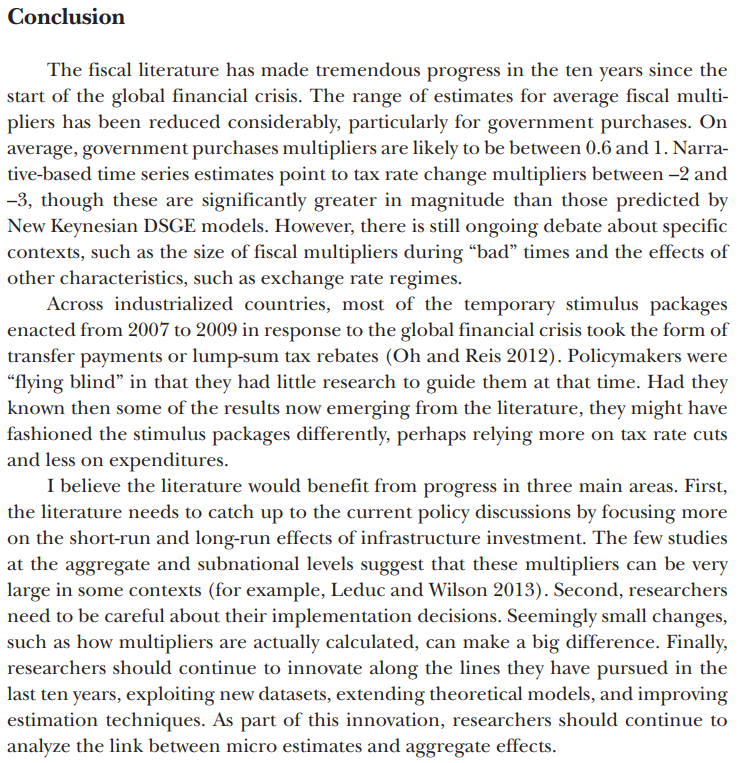
\includegraphics[width=5cm]{./figures/aula9_fig3.PNG}}            
            }
           \end{tabular} \\
    \end{tabular}
\end{frame}

\begin{frame}
    {Introdução}
    \begin{figure}
        \centering
        \href{https://www.bcb.gov.br/publicacoes/agenda_pesq_macro}{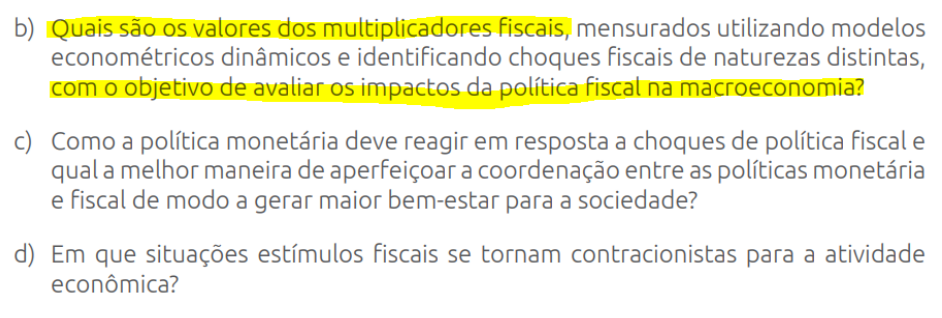
\includegraphics[width=\textwidth]{./figures/aula9_fig1.PNG}}
        \caption{Agenda de pesquisa BCB (2021-2024). Fonte: \href{https://www.bcb.gov.br/publicacoes/agenda_pesq_macro}{Banco Central do Brasil: Política fiscal e seus efeitos}}
    \end{figure}
\end{frame}

\section{Fatores que afetam o multiplicador}
\begin{frame}
    {Fatores que afetam o multiplicador}
    \begin{itemize}
        \item A hipótese da renda permanente prediz que o tamanho do multiplicador depende do grau de permanência de um choque de renda\bigskip
        \item A propensão marginal a consumir de um choque temporário e não-antecipado de renda é próximo ao tamanho da taxa de juros, i.e., apenas $\frac{r}{1 + r}$\bigskip
        \item Portanto, prediz-se que o multiplicador seja próximo à unidade para choques temporários de renda\bigskip
        \item Por outro lado, choques permanentes de renda irão resultar em um multiplicador maior que um à medida que famílias revisam suas decisões de consumo de maneira a refletir uma nova renda permanente mais elevada
    \end{itemize}
\end{frame}

\begin{frame}
    {Fatores que afetam o multiplicador}
    \begin{itemize}
        \item A presença de restrições de crédito e consumidores impacientes também impactam o tamanho do multiplicador\bigskip
        \item Para este tipo de consumidor, o efeito multiplicador será maior que 1 mesmo quando o choque de renda é temporário, dado que suas propensões marginais a consumir são iguais a 1\bigskip
        \item Quanto maior a fração de agentes \emph{hand-to-mouth} ou \emph{rule-of-thumb} na economia, maior será o multiplicador
    \end{itemize}
\end{frame}

\begin{frame}
    {Fatores que afetam o multiplicador}
    \begin{itemize}
        \item Incerteza a respeito da permanência de choques de renda é um outro fator que influencia o multiplicador\bigskip
        \item Se uma fração substancial das flutuações observadas na renda são percebidas como permanentes, então, isto resultará em um multiplicador maior que 1\bigskip
        \item Neste caso, consumidores podem ainda seguir a hipótese da renda permanente, no entanto, a incerteza leva seu comportamento a ser compatível com a função de consumo Keynesiana\bigskip
        \item \textcolor{purple}{Uma variação no multiplicador irá deslocar a curva IS e alterar sua inclinação} (um multiplicador mais elevado torna IS mais plana)
    \end{itemize}
\end{frame}

\section{Outros fatores que afetam inclinação da IS}
\begin{frame}
    {Outros fatores que afetam a inclinação da curva IS}
    \begin{itemize}
        \item Além do efeito do tamanho do multiplicador, a inclinação da curva IS também é afetada pela sensibilidade do investimento e do consumo a variações na taxa de juros\bigskip
        \item A predição teórica de um impacto da taxa de juros sobre o consumo é ambígua: uma redução na taxa de juros estimula o consumo através de alguns canais (efeito riqueza) e amortece através de outros\bigskip
        \item A evidência empírica da função consumo sugere que as estruturas institucionais nacionais, particularmente no que diz respeito ao sistema financeiro, são importantes na determinação da força e direção desta relação\bigskip        
    \end{itemize}
\end{frame}

\begin{frame}{Outros fatores que afetam a inclinação da curva IS}
    \begin{tabular}{cl}
        \begin{tabular}{c}
            \href{https://onlinelibrary.wiley.com/doi/abs/10.1111/j.1475-4991.2011.00466.x}{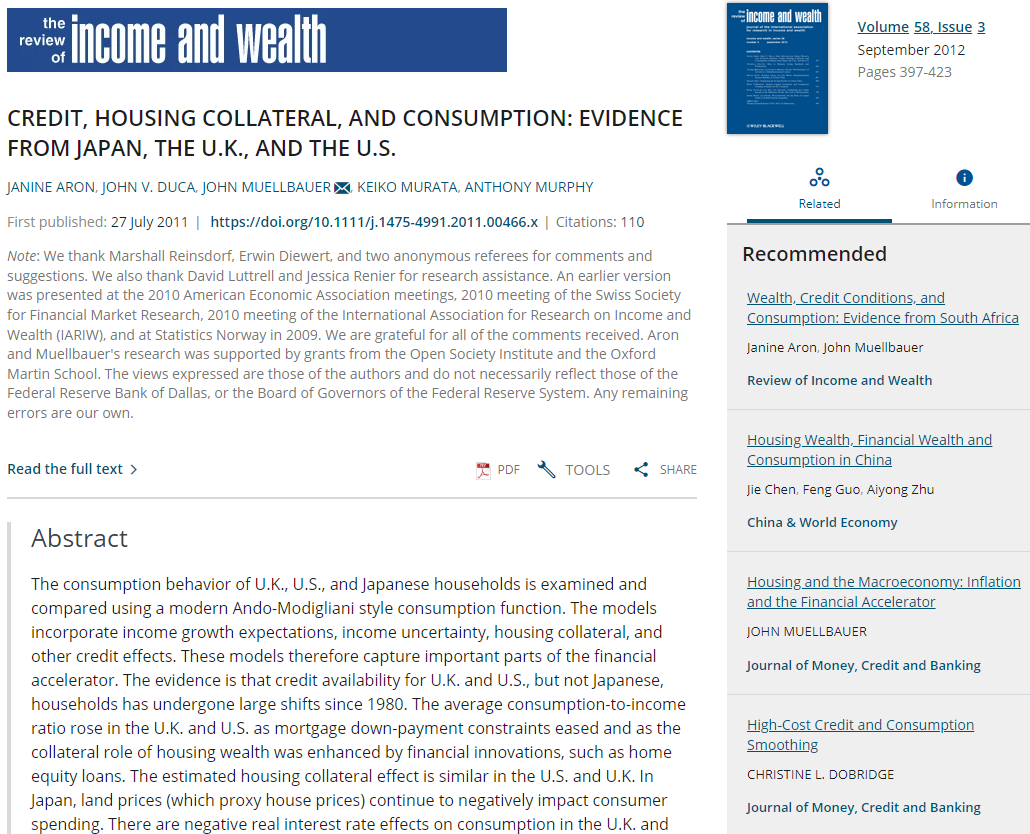
\includegraphics[width=5cm]{./figures/aula9_fig5.PNG}}            
        \end{tabular}
         & \begin{tabular}{l}
               \parbox{0.6\linewidth}{%  change the parbox width as appropiate
                   \begin{itemize}
                    \item \href{https://onlinelibrary.wiley.com/doi/abs/10.1111/j.1475-4991.2011.00466.x}{Aron et al. (2012)} encontraram uma relação negativa entre consumo e taxa real de juros em economias com maior liberalização financeira como UK e EUA\bigskip
                    \item Mas encontraram uma relação positiva no Japão, onde enormes depósitos líquidos das famílias mais que compensam suas dívidas
                    \end{itemize}
               }
           \end{tabular} \\
    \end{tabular}
\end{frame}

\begin{frame}
    {Outros fatores que deslocam a curva IS}
    \begin{itemize}
        \item Além dos efeitos do tamanho do multiplicador, a curva IS pode ser deslocada por um conjunto de outros fatores\bigskip
        \item Consumo: HRP prediz que qualquer fator que altere a riqueza esperada ao longo do ciclo de vida, $\Psi_t^e$, como mudanças no preço de ativos ou notícias de uma promoção futura, deslocam a curva IS\bigskip
        \item As evidências empíricas de consumo destacam três outros fatores que podem deslocar a curva IS
    \end{itemize}
\end{frame}

\begin{frame}
    {Outros fatores que deslocam a curva IS}
    \begin{enumerate}
        \item Incerteza: aumento na taxa de desemprego, e.g., aumenta poupança precaucionária, deslocando IS para esquerda\medskip
        \item \emph{Boom} no preço de imóveis em países com empréstimos do tipo \emph{home equity}\footnote{Crédito com garantia de imóvel: empréstimos com taxas de juros menores que as praticadas no mercado} afrouxa restrições de crédito, deslocando IS para direita. No entanto, um \emph{boom} no preço de imóveis pode também deslocar curva IS para a esquerda em países onde empréstimos de \emph{home equity} são inacessíveis e, portanto, grandes adiantamentos são necessários para conseguir uma hipoteca\medskip
        \item Deslocamentos na arquitetura do mercado de crédito que aumentam acesso a crédito para famílias (inovações financeiras e/ou desregulamentações) deslocam IS para a direita (pelo menos até o ponto em que o acúmulo de dívidas eventualmente cancele parte do deslocamento)
    \end{enumerate}
\end{frame}

\begin{frame}
    {Outros fatores que deslocam a curva IS}
    \begin{itemize}
        \item Investimento - $q$ marginal de Tobin prediz que os seguintes fatores deslocam IS para direita:\bigskip
        \begin{enumerate}
            \item Aumento no preço do produto, $P$\medskip
            \item Aumento na produtividade marginal do capital, $F_K$\medskip
            \item Redução na taxa de depreciação do capital, $\delta$\bigskip
        \end{enumerate}
        \item Por fim, a equação de $Q$ médio destaca o papel das expectativas de lucros futuros como fator de deslocamento da IS\bigskip
        \item Aumento no mercado de ações tende a estimular investimentos, pois sinaliza aumento no valor das companhias relativo aos custos de reposição
    \end{itemize}
\end{frame}

\section{Considerações finais}
\begin{frame}
    {Considerações finais}
    \begin{itemize}
        \item Curva IS possibilita pensar, sistematicamente, como variações no comportamento dos gastos de firmas, famílias e governo podem influenciar o produto agregado e determinar o ciclo econômico\bigskip
        \item Curva IS mostra combinações de taxa real de juros e produto agregado que equilibram o mercado de bens e serviços\bigskip
        \item É negativamente inclinada, representando o fato de que decisões de consumo por parte das famílias responde negativamente à taxa de juros e, além disso, as firmas também irão incorrer em novos projetos de investimento à medida que o custo dos empréstimos aumenta
    \end{itemize}
\end{frame}

\begin{frame}
    {Considerações finais}
    \begin{enumerate}
        \item Se um indivíduo recebe um bônus de \$100, quanto deste bônus irá ser revertido em consumo?\bigskip
        \item De quanto será o aumento no produto agregado após um aumento de demanda autônoma como gastos do governo mais elevados ou aumento na confiança de famílias e firmas?\bigskip
        \item Em que medida um aumento na taxa de juros irá impactar as decisões de investimento?
    \end{enumerate}
\end{frame}

\begin{frame}
    {Considerações finais}
    \begin{itemize}
        \item Nas últimas aulas desenvolvemos um modelo de lado de demanda que nos ajuda a compreender algumas questões macro\bigskip
        \item Modelos de consumo e investimento que se relacionam com características observáveis do mundo real\bigskip
        \item E.g., a maior volatilidade do investimento comparado ao consumo pode ser, parcialmente, explicada por fatores que influenciam as decisões de gastos com $I$ e por consumidores que tomam empréstimos e poupam para suavizar consumo ao longo do ciclo econômico\bigskip
        \item Existência de heterogeneidade entre consumidores: alguns são impacientes e têm dificuldade de poupar, outros são prudentes e poupam por motivos precaucionários, etc.
    \end{itemize}
\end{frame}

\begin{frame}
    {Considerações finais}
    \begin{itemize}
        \item Governo contribui para suavização de consumo via estabilizadores automáticos, como seguro-desemprego\bigskip
        \item Restrições de crédito (consumidores e firmas) ajuda a melhor alinhar modelos de consumo e investimento com evidências empíricas\bigskip
        \item Lado da demanda tem grande influência sobre a atividade econômica. No entanto, é apenas um dos componentes que ajuda a explicar o funcionamento da macro\bigskip
        \item Para compreendermos flutuações econômicas e tendências de médio/longo prazo, precisamos introduzir o lado da oferta ao nosso modelo\bigskip
        \item Com isso, poderemos entender como salários e preços são determinados e o que determina a taxa de desemprego\bigskip
        \item Este será nosso próximo objeto de estudo
    \end{itemize} 
\end{frame}

\section{Bibliografia}
\begin{frame}{\emoji{books} Bibliografia}
    \begin{itemize}        
        \item ARON, J.; DUCA, J.V.; MUELLBAUER, J.; BAUER, J.; MURATA, K.; MURPHY, A. Credit, housing collateral, and consumption: Evidence from Japan, the UK and the US. \emph{Review of Income and Wealth}, 58(3): 397-423, 2012\medskip
        \item BLANCHARD, O. Macroeconomia. 7.ed. São Paulo: Pearson Education do Brasil, 2017\medskip                
        \item CARLIN, W.; SOSKICE, D. Macroeconomics: Institutions, instability, and the financial system. Oxford, UK: Oxford University Press, 2015\medskip
        \item CHALLE, E. Macroeconomic fluctuations and policies. Cambridge, MA: The MIT Press, 2019\medskip        
        \item RAMEY, V. A (2019). "Ten Years after the Financial Crisis: What Have We Learned from the Renaissance in Fiscal Research?" Journal of Economic Perspectives, 33 (2): 89-114\medskip
        \item UHLIG, H (2010). "Some Fiscal Calculus." American Economic Review, 100 (2): 30-34
    \end{itemize}
\end{frame}
\end{document}